\documentclass[10pt, aspectratio=169]{beamer}

\input{settings/special_beamer}
\usepackage[T2A]{fontenc}
\usepackage[utf8]{inputenc}
\usepackage[english, russian]{babel}
\usepackage{hyperref}     % ТАК_НУЖНО
\hypersetup{unicode=true} % ТАК_НУЖНО
\usepackage{amsmath}
\usepackage{amssymb,textcomp, esvect,esint}
\usepackage{amsfonts}
\usepackage{amsthm}
\usepackage{graphicx}
\usepackage{indentfirst}
\usepackage{xcolor}
% \usepackage{enumitem} %--- ломал нумерацию!?

\usepackage{graphicx}
\usepackage{booktabs}
\usepackage{caption}
\usepackage{listings}
\usepackage{tikz}
\usepackage{xcolor}
\usepackage{cancel}


\usepackage[justification=justified]{caption}

% \usepackage{media9}
% \usepackage{animate}
% \usepackage{threeparttable}
% \usepackage{pifont}


\usepackage{import}
\usepackage{xifthen}
\usepackage{pdfpages}
\usepackage{transparent}

% \usepackage{natbib}

\usepackage[skip=1pt]{caption}

\usepackage{ifthen}
\definecolor{darkgreen}{RGB}{10,90,10}
\definecolor{crane}{RGB}{255,187,3}
\definecolor{seahorse}{RGB}{215,211,233}

% \usetikzlibrary{tikzmark,fit,shapes.geometric} % рисование кружочков


\usepackage{subfigure}

\newcommand{\kB}{k_{\textnormal{B}}}
\newcommand{\vcap}{\sub{v}{c}}
\newcommand{\dC}{\,{}^\circ\textnormal{С}}


\newcommand{\incfig}[1]{%
    % \def\svgwidth{\columnwidth}
    \import{figures/}{#1.pdf_tex}
}

% \usepackage{circuitikz}

\newcommand{\vc}[1]{\mbox{\boldmath $#1$}}
\newcommand{\smallvc}[1]{\scalebox{0.65}{\mbox{\boldmath $#1$}}}

\newcommand{\T}{^{\text{T}}}
\newcommand{\R}{\text{R}}
\newcommand{\const}{\text{const}}
\newcommand{\sub}[2]{#1_{\textnormal{#2}}}
% \renewcommand{\tg}{\mathop{\mathrm{tg}}\nolimits}

\renewcommand{\Im}{\mathop{\mathrm{Im}}\nolimits}
\renewcommand{\Re}{\mathop{\mathrm{Re}}\nolimits}
\renewcommand{\d}{\, d}
\renewcommand{\leq}{\leqslant}
\renewcommand{\geq}{\geqslant}

\newcommand{\cmark}{\text{\ding{51}}}
\newcommand{\xmark}{\text{\ding{55}}}



\definecolor{mygray}{gray}{0.6}
\definecolor{mygreen}{RGB}{8,99,44}
\definecolor{myred}{RGB}{164,0,0}



\newcommand{\iitem}[1]{\item[\textcolor{myred}{\scalebox{0.7}{$\blacksquare$}}]{#1}}
\title[Оптимизация в МОЛ]{Оптимизация количества атомов тулия \\ в
магнито-оптической ловушке}


\author[Хоружий Кирилл]{Хоружий Кирилл \texorpdfstring{
\\
\phantom{}\\
группа <<Квантовые симуляторы и интегрированная фотоника>>\\
\phantom{}\\
Научный руководитель: Акимов А. В. \\
Научный консультант: Цыганок В. В.
}{} 
}
\institute[РКЦ, МФТИ]


\let\tg\undefined %костыль связанный с русским языком и tg

\setbeamertemplate{caption}[numbered]

\begin{document}
\maketitle


\frame{
	


\begin{minipage}{0.25\textwidth}
Квантовые приборы:
\begin{itemize}
	\iitem{гравиметры}
	\iitem{часы}
	\iitem{транспортиры}
	\iitem{...}
	\iitem{...}
\end{itemize}
\end{minipage}
\hfill
\begin{minipage}{0.7\textwidth}
\textbf{Квантовые симуляторы}:
\begin{itemize}
	\iitem{реализация моделей ферми-хаббарда и бозе-хаббарда}
	\iitem{переход от БКШ к БЭК}
	\iitem{локализация Андерсона и многочастичная локализация}
	\iitem{формирование вихрей в БЭК}
	\iitem{...}
\end{itemize}
\end{minipage}


\phantom{42}

\phantom{42}



 \frametitle{Ультрахолодные газы}
}
\frame{
	\only<1>{
\begin{figure}[h]
        \centering
        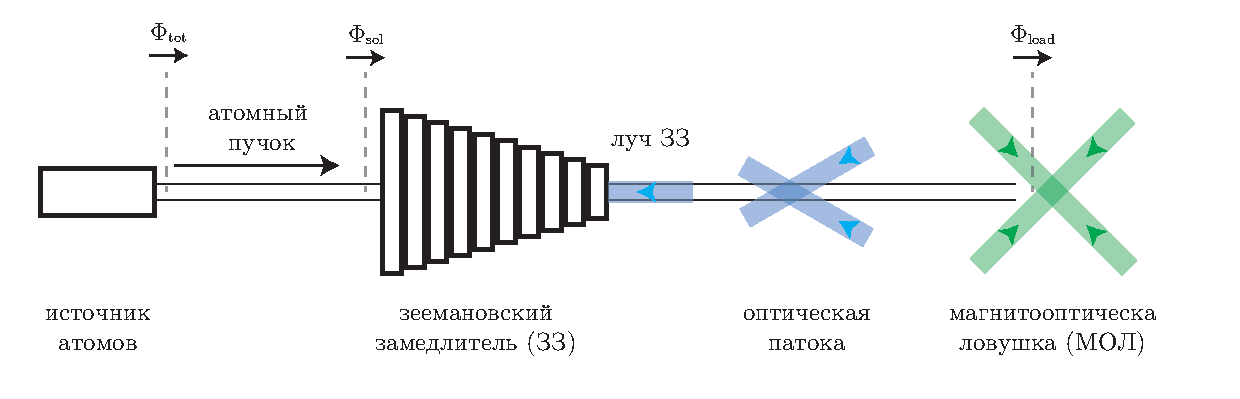
\includegraphics[width=0.68\textwidth]{../MOT/figs/sheme.pdf}
        \caption{Принципиальная схема установки}
    \end{figure}

    \begin{figure}[h]
        \centering
        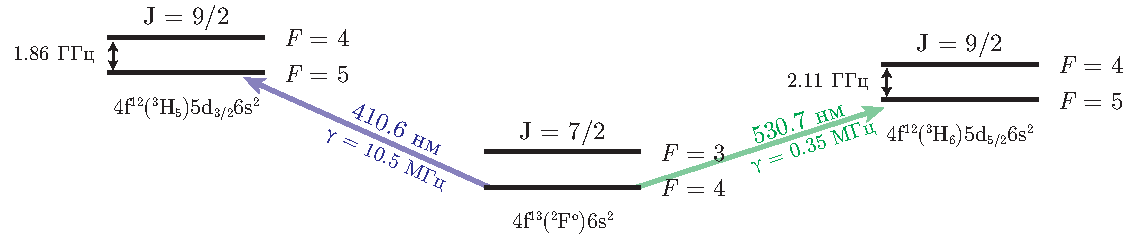
\includegraphics[width=0.68\textwidth]{../MOT/figs/tm_pres.pdf}
        \caption{Используемые в эксперименте атомные переходы}
    \end{figure}
}

\only<2>{
\begin{minipage}{0.68\textwidth}
    \begin{figure}[h]
        \centering
        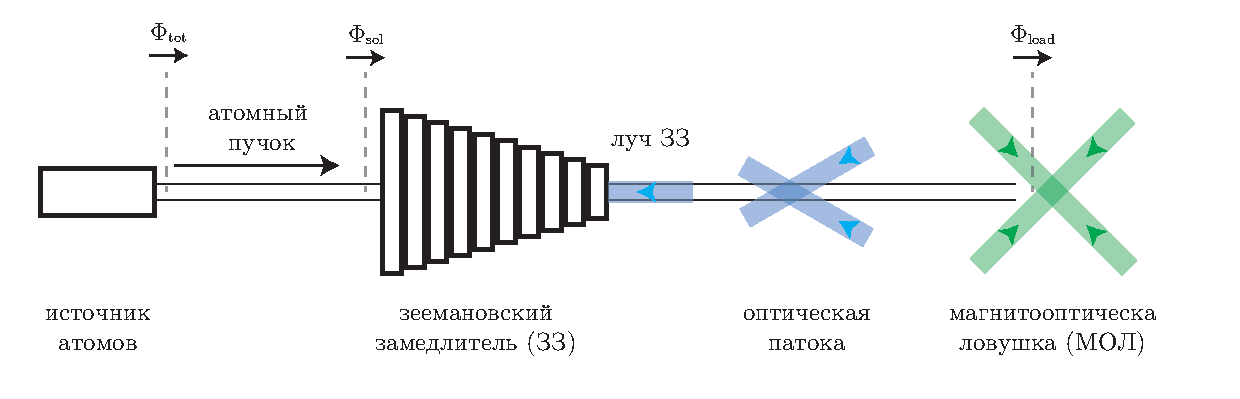
\includegraphics[width=1.0\textwidth]{../MOT/figs/sheme.pdf}
        \caption{Принципиальная схема установки}
    \end{figure}

    \begin{figure}[h]
        \centering
        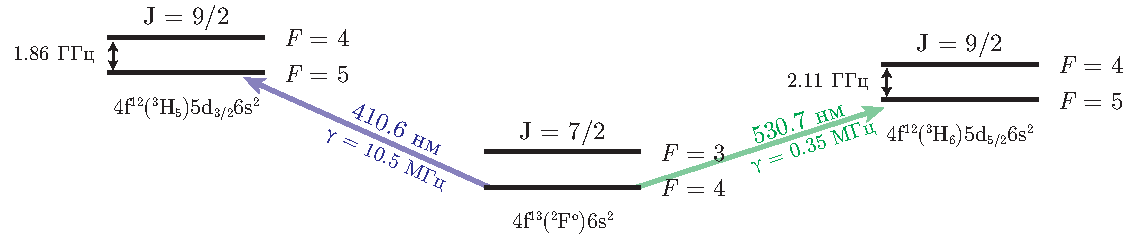
\includegraphics[width=1.0\textwidth]{../MOT/figs/tm_pres.pdf}
        \caption{Используемые в эксперименте атомные переходы}
    \end{figure}
\end{minipage}
\hfill
\begin{minipage}{0.31\textwidth}

$\sub{t}{life}$ -- время непрерывной \\ работы установки

\phantom{42}


Ограничения на $\sub{t}{life}$:
\begin{itemize}
    \iitem{заканчиваются атомы}
    \iitem{напыление на зеркало перед замедлителем}
\end{itemize}

\phantom{42}

\textbf{Задача}: \\ увеличить $\sub{t}{life}$, сохранив $\sub{\Phi}{load}$


\end{minipage}
}
\only<3>{
\begin{minipage}{0.68\textwidth}
    \begin{figure}[h]
        \centering
        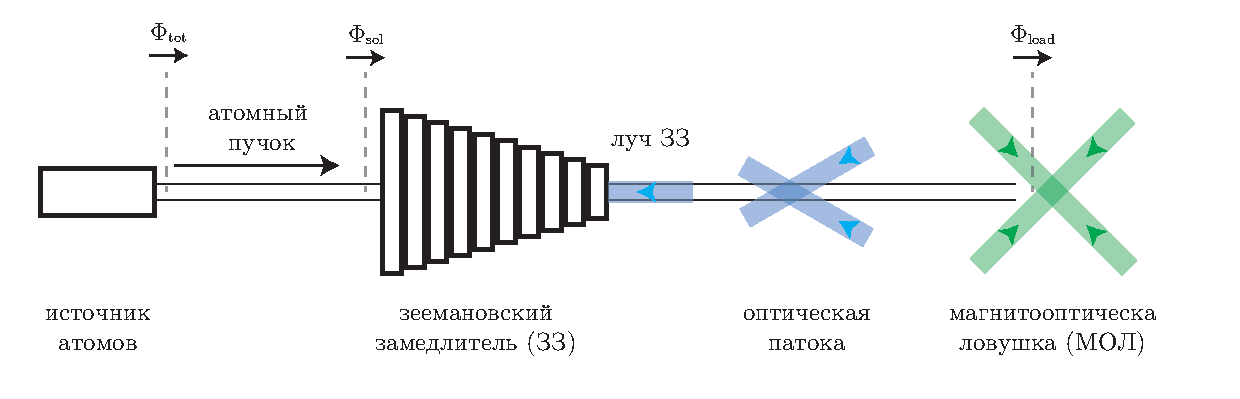
\includegraphics[width=1.0\textwidth]{../MOT/figs/sheme.pdf}
        \caption{Принципиальная схема установки}
    \end{figure}

    \begin{figure}[h]
        \centering
        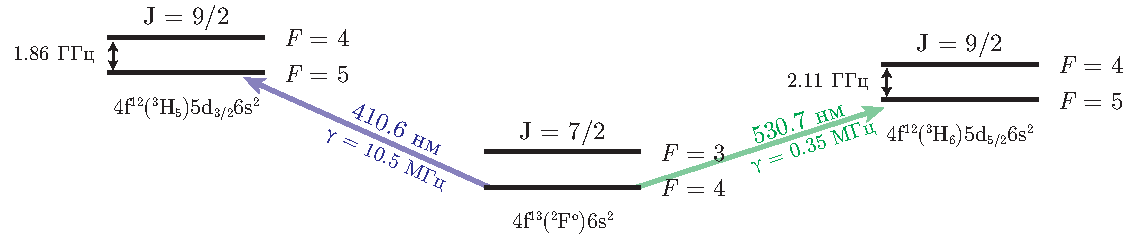
\includegraphics[width=1.0\textwidth]{../MOT/figs/tm_pres.pdf}
        \caption{Используемые в эксперименте атомные переходы}
    \end{figure}
\end{minipage}
\hfill
\begin{minipage}{0.31\textwidth}
\textbf{Задача}: \\ увеличить $\sub{t}{life}$, сохранив $\sub{\Phi}{load}$

\begin{align*}
    \sub{t}{life} &\propto 1/\sub{\Phi}{tot}(T) \\    
    \sub{\Phi}{sol} &\propto \, \sub{\Phi}{tot} \\ 
    \sub{\Phi}{load} &= \eta\, \sub{\Phi}{sol}
\end{align*}

$\eta$ -- эффективность ЗЗ

\phantom{42}


Дальнейшие действия:
\begin{itemize}
    \iitem{понижение $T$}
    \iitem{ повышение $\eta$}
\end{itemize}

\end{minipage}
}
   


 \frametitle{Общая схема охлаждения}
}
\frame{
	


\begin{minipage}{0.65\textwidth}

\begin{figure}[ht]
    \centering
    \includegraphics[width=0.9\textwidth]{../MOT/figs/Bz_v2.pdf}
    \caption{Зависимость магнитного поля внутри зеемановского замедлителя от координаты $z$. Ток маленькой катушки $\sub{I}{small} = 17\,$А, ток большой катушки $\sub{I}{big} = 35\,$А.}
\end{figure}


\end{minipage}
\hfill
\begin{minipage}{0.31\textwidth}

Тормозящая сила:
\begin{equation*}
    F = \frac{\hbar k \Gamma}{2} \frac{s}{1+s+4({\delta}+k v)^2/\Gamma^2}
\end{equation*}

\phantom{42}

Эффект Доплера:\\
\phantom{42} \hfill
$1\,\text{м}/\text{с} \sim 2\,\text{МГц}$

При этом: \\
\phantom{42} \hfill
$\Gamma \sim 10\,\text{МГц}$

Замедление \\
\phantom{4} 
от $150\,\text{м}/\text{с}$ до $\sub{v}{slow} \sim 30\,\text{м}/\text{с}$

\phantom{42}



Необходима подстройка резонанса магнитным полем:
\begin{equation*}
    \delta \to \delta + \mu B / \hbar
\end{equation*}


\end{minipage} \frametitle{Зеемановский замедлитель I}
}
\frame{
	

% \begin{tikzpicture}[remember picture,overlay]    \draw[seahorse] (10.5,0.75) -- (10.5,-6.75); \end{tikzpicture}


\begin{minipage}{0.65\textwidth}

\begin{figure}[ht]
    \centering
    \subfigure[]{\includegraphics[scale=0.7]{../MOT/figs/vz_v2.pdf}}
    \hspace{5 mm} 
    \subfigure[]{\includegraphics[scale=0.7]{../MOT/figs/vdist_v5.pdf}}
    % zeeman_sim_v2
    \caption{a) Зависимость скорости атомов от координаты в зеемановском замедлителе  для различных начальных скоростей. б) Характерное преобразование распределения атомов по скоростям после замедления. }
\end{figure}


\end{minipage}
\hfill
\begin{minipage}{0.31\textwidth}

Тормозящая сила:
\begin{equation*}
    F = \frac{\hbar k \Gamma}{2} \frac{s}{1+s+4({\delta}+k v)^2/\Gamma^2}
\end{equation*}

\phantom{42}

Уравнение движения:
\begin{equation*}
    \frac{d v}{d t} = \frac{F}{m},
    \hspace{0.1cm} \overset{v \d t = \d z}{\Leftrightarrow}  \hspace{0.1cm}
    \frac{d v}{d z} = \frac{F(v, z)}{m \, v(z)}
\end{equation*}



\end{minipage} \frametitle{Зеемановский замедлитель II}
}
\frame{
	



\begin{minipage}{0.65\textwidth}
\begin{figure}[ht]
    \centering
    \rotatebox{90}{\hspace{8mm}\scalebox{0.8}{$B_0=700\un{Гс}$ \hspace{16 mm} $B_0=300\un{Гс}$}}
    \hspace{1 mm} 
    \includegraphics[width=0.94\textwidth]{../MOT/figs/etas_v4.pdf}
    \caption{Зависимость эффективности работы замедлителя $\eta$ от отстройки луча ЗЗ $\delta$, параметра насыщения $s$ для двух различных значений амплитуды магнитного поля в ЗЗ}
\end{figure}

\end{minipage}
\hfill
\begin{minipage}{0.31\textwidth}



Загрузка в МОЛ: $\ v < \sub{v}{cap}$

\phantom{42}

$\eta = \frac{\sub{\Phi}{load}}{\sub{\Phi}{sol}}$ -- эффективность ЗЗ

\phantom{42}

\begin{figure}[h]
    \centering
    \includegraphics[scale=0.66]{../MOT/figs/vdist_v5.pdf}
    \caption{Преобразование распределения атомов по скоростям после ЗЗ}
    %\label{fig:}
\end{figure}


\end{minipage} \frametitle{Зеемановский замедлитель III}
}
\frame{
	\begin{minipage}{0.68\textwidth}




\only<1>{

Сила в МОЛ:
	\begin{equation*}
		\vc{F} = \frac{\hbar \vc{k} \Gamma}{2}\left(
			\frac{s}{1+s+4\left(\frac{2\pi \delta - \vc{k} \vc{v}}{\Gamma}\right)^2}-
			\frac{s}{1+s+4\left(\frac{2\pi \delta + \vc{k} \vc{v}}{\Gamma}\right)^2}
		\right)
	\end{equation*}

	\begin{figure}[h]
    \centering
    \includegraphics[width=0.8\textwidth]{../MOT/figs/motF.pdf}
    \caption{Зависимость ускорения от силы светового давления, действующей на движущийся атом от его скорости}
    %\label{fig:}
\end{figure}
}

\only<2>{

Сила в МОЛ:
	\begin{equation*}
		\vc{F} = \frac{\hbar \vc{k} \Gamma}{2}\left(
			\frac{s}{1+s+4\left(\frac{2\pi \delta - \vc{k} \vc{v}}{\Gamma}\right)^2}-
			\frac{s}{1+s+4\left(\frac{2\pi \delta + \vc{k} \vc{v}}{\Gamma}\right)^2}
		\right)
	\end{equation*}

	Магнитное поле $\Rightarrow$ эффект Зеемана:
	\begin{equation*}
		\vc{B} = \beta (-x,\,  -y,\, 2z)\T/2,
		\hspace{10 mm} 
		\Delta E = - \vc{B} \vc{\mu},
		\hspace{5 mm} 
		\delta \to \delta + \Delta E /\hbar
	\end{equation*}

	\phantom{42}



	Движение в МОЛ $\sim$ затухающий осциллятор:
	\begin{equation*}
		\vc{F}(\vc{r}, \vc{v}) = -\alpha \vc{v} - \varkappa \vc{r}
	\end{equation*}

	с коэффициентами
	\begin{equation*}
			\varkappa = \frac{-\delta}{\Gamma/2\pi}\frac{8 \subt{\mu}{B} \beta k s}{\left(1+s+4\left(\frac{2\pi \delta}{\Gamma}\right)^2\right)^2},
			\hspace{5 mm} 
			\alpha = \frac{-\delta}{\Gamma} \frac{8 \hbar k^2 s}{\left(1+s+4\left(\frac{2\pi \delta}{\Gamma}\right)^2\right)^2},
	\end{equation*}

}



\end{minipage}
\hfill
\begin{minipage}{0.31\textwidth}

\begin{figure}[h]
    \centering
    \includegraphics[width=1.0\textwidth]{../MOT/figs/mot.png}
    \caption{Схема лучей МОЛ}
    %\label{fig:}
\end{figure}

\end{minipage}



 \frametitle{Магнито-оптическая ловушка (МОЛ)}
}
\frame{
	% \begin{figure}[ht]
%     \centering
%     \includegraphics[width=0.6\textwidth]{../MOT/figs/fit_mot_v2.pdf}
%     \caption{Экспериментально сфотографированное распределение 
%     атомов $\sub{f}{exp}$ и аппроксимация распределения атомов $\sub{f}{fit}$
%     }
% \end{figure}

\begin{minipage}{0.68\textwidth}
Закон Бугера-Ламберта-Бера:
\begin{equation*}
    \frac{d I}{d z} = - \sigma n I,
    \hspace{10 mm} 
    \sigma = \frac{\sigma_0}{1+I/I_s + 4 (\delta/\Gamma)^2},
\end{equation*}


Распределение интенсивности:
\begin{equation*}
    \sub{f}{exp} = \ln\left(\frac{\subt{I}{D}}{I_0}\right) + \frac{\subt{I}{D} - I_0}{I_s} = \sigma_0 \int n(x, y, z) \d z.
\end{equation*}

\begin{figure}[ht]
    \centering
    \includegraphics[width=0.9\textwidth]{../MOT/figs/detect.png}
    \caption{Схема детектирования атомов}
\end{figure}
\end{minipage}
\hfill
\begin{minipage}{0.31\textwidth}

$\subt{I}{D}$ -- фотография без атомов

$\sub{I}{0}$ -- фотография с атомами

$\sub{I}{s}$ -- интенсивность насыщения

\begin{figure}[h]
    \centering
    \includegraphics[width=0.99\textwidth]{../MOT/figs/fit_mot_v4.pdf}
    \caption{Фото распределения}
    %\label{fig:}
\end{figure}


\end{minipage} \frametitle{Фотографирование атомов}
}
\frame{
	\begin{minipage}{0.6\textwidth}

Аппроксимация распределения:
\begin{equation*}
    \sub{f}{fit}(x, y) = B+A \exp\left(
        - \left(\frac{\tilde{x}}{\sigma_1}\right)^2 - \left(\frac{\tilde{y}}{\sigma_2}\right)^2
    \right)
\end{equation*}


\end{minipage}
\hfill
\begin{minipage}{0.31\textwidth}

Полное число атомов:
\begin{equation*}
\boxed{
	N = \pi A \sigma_1 \sigma_2
}
\end{equation*}

\end{minipage}


\begin{figure}[h]
    \centering
    \includegraphics[width=0.8\textwidth]{../MOT/figs/fit_mot_v2.pdf}
    \caption{Экспериментально сфотографированное распределение атомов $\sub{f}{exp}$, аппроксимация распределения атомов гауссовой функцией $\sub{f}{fit}$ и остатки аппроксимации $|\sub{f}{exp} - \sub{f}{fit}|$}
    %\label{fig:}
\end{figure}
 \frametitle{Количество атомов в МОЛ}
}
\frame{
	Динамика количества атомов в МОЛ:
\begin{equation*}
	\frac{d N}{d t} = \sub{\Phi}{load} - \cancel{\gamma N} - \beta N^2
	\hspace{0.5cm} \Rightarrow \hspace{0.5cm}
	N(t) = \sqrt{\frac{\sub{\Phi}{load}}{\beta}} \left(1-e^{-t \sqrt{\beta \sub{\Phi}{load}}}\right)
\end{equation*}




\begin{minipage}{0.6\textwidth}


\begin{figure}[h]
    \centering
    \includegraphics[width=0.8\textwidth]{../MOT/figs/motload_v2.pdf}
    \caption{Динамика загрузки МОЛ для различных значений отстройки $\delta$ лучей МОЛ}
    %\label{fig:}
\end{figure}

\end{minipage}
\hfill
\begin{minipage}{0.35\textwidth}

\begin{figure}[h]
    \centering
    \includegraphics[width=0.8\textwidth]{../MOT/figs/motload2_v2.pdf}
    \caption{Зависимость максимального числа атомов в МОЛ от величины отстройки $\delta$ лучей МОЛ}
\end{figure}

\end{minipage} \frametitle{Загрузка МОЛ: оптимизация отстройки лучей МОЛ}
}
\frame{
	\begin{figure}[ht]
    \centering
    \subfigure[]{\includegraphics[width=0.3\textwidth]{../MOT/figs/IZ1.pdf}}
    \hspace{10 mm} 
    \subfigure[]{\includegraphics[width=0.6\textwidth]{../MOT/figs/IZ2.pdf}}
    \caption{a) Зависимость количества загруженных за 5с в МОЛ атомов от величины токов малой и большой катушки ЗЗ. Зависимость снята  при оптимальной отстройке лучей ОП $\subt{\delta}{ОП}$. 
    б) Зависимость количества загруженных за 5с при оптимальной отстройке лучей ОП в МОЛ атомов от величины токов малой и большой катушки ЗЗ. Зависимость снята при $\subt{\delta}{ОП}$ большей и меньшей оптимального значения в $\subt{\delta}{ОП} = 9.4 \Gamma$.}
\end{figure}

 \frametitle{Загрузка МОЛ: оптимизация токов зеемановского замедлителя}
}
\frame{
	\begin{minipage}{0.65\textwidth}
    \vspace{-1mm}

    \begin{figure}[h]
        \centering
        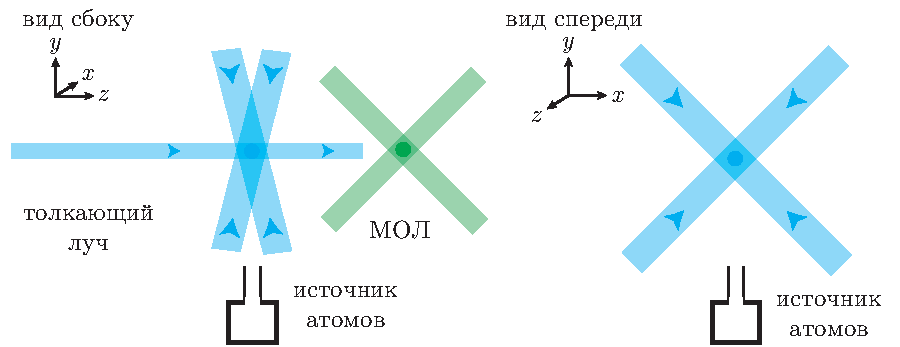
\includegraphics[width=0.9\textwidth]{../MOT/figs/2dmot_v3.pdf}
        \vspace{1mm}
        \caption{Принципиальная схема лучей 2D-МОЛ}
        \label{fig:2dmots}
    \end{figure}

    \vspace{-8mm}

    \begin{figure}[h]
        \centering
        \includegraphics[width=1.0\textwidth]{../MOT/figs/vcap2d_delta-Ds.png}
        \caption{Зависимость скорости захвата 2D-МОЛ для различных мощностей от отстройки $\delta$ лучей 2D-МОЛ и размера $D$ пучков}
    \end{figure}
\end{minipage}
\hfill
\begin{minipage}{0.31\textwidth}

Загрузка МОЛ: \vspace{-3mm}
\begin{align*}
    % \sub{\Phi}{load} &\propto \sub{\Phi}{tot} \int_{0}^{\vcap} v^3 e^{-v^2/\alpha^2} \d v \\
    \sub{\Phi}{load} &\propto  \sub{\Phi}{sol} \left(\frac{\sub{v}{\textcolor{blue}{cap}}}{\alpha}\right)^4
\end{align*}


Скорости захвата: \vspace{-3mm}
\begin{equation*}
    m \int_{\vcap}^{0} \frac{v}{F(v)} \d v = D
\end{equation*}


Критическое расстояние: \vspace{-3mm}
\begin{equation*}
    \sub{l}{крит} \sim \sqrt{\frac{\sub{h}{крит} \sub{v}{\textcolor{green}{cap}}^2}{g}} \sim 1\,\text{м}
\end{equation*}


\phantom{42}

При $T \sim 700 \dC$: \\ 
$\sub{\Phi}{load}(\sub{v}{\textcolor{blue}{cap}} = 40\,\text{м/c}) \sim 10^8\,\text{c}^{-1}$

\end{minipage} \frametitle{2D-MOЛ}
}
\frame{
	% Тут что-то в духе

%  было: ...


%  стало: ...


%  Стало лучше!

%  

\begin{itemize}
	\iitem{Построена модель ЗЗ. Моделированием методом Монте-Карло определена зависимость системы от параметров.}
	\iitem{Оптимизацией работы ЗЗ, ОП и МОЛ удалось уменьшить температуру с $730\dC$ до $680\dC$, сохранив загрузку МОЛ $\sub{\Phi}{load}$ на исходном уровне. Это увеличило время непрерывной работы установки в 5 раз: с 2 месяцев до 10 месяцев.} 
	\iitem{Подготовлена альтернатива ЗЗ: 2D-МОЛ. Произведены основные оценки необходимые для работы 2D-МОЛ. После 2D-МОЛ мы можем получить загрузку МОЛ $\sub{\Phi}{load}$ на исходном уровне, таким образом 2D-МОЛ является компактной перспективной заменой ЗЗ.}
\end{itemize}



 \frametitle{Заключение}
}
\frame{
	\centering
\LARGE{Спасибо за внимание!} \frametitle{}
}


\end{document}



